\subsection{Excited \emph{$D_{(s)}$} mesons}

Tables \ref{table:charm:spect:1} and \ref{tabel:charm:spect:2} summarize recent measurements of the masses and widths of $D_{s}$ and $D$ mesons, respectively. If a preferred assignment of spin and parity was measured it is listed in the column $J^{P}$, where the label natural denotes $J^{P}=0^{-},1^{+},2^{-}\ldots$ and unnatural $J^{P}=0^{+},1^{-},2^{+}\ldots$. If possible an average mass and width was calculated, which is listed in the gray shaded row. The calculation of the averages assumes no correlation between individual measurements. A summary of the averaged masses and widths is shown in Figure~\ref{fig:charm:spect:1}. 
\begin{figure}[htb!]
\begin{centering}
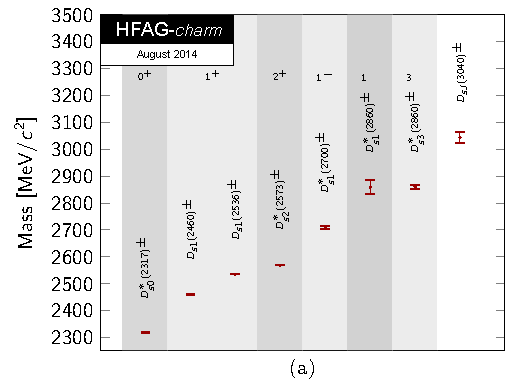
\includegraphics[width=0.45\textwidth]{./figures/charm/Dsmasses}
\quad
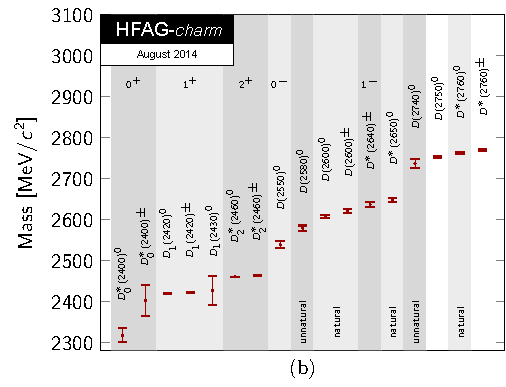
\includegraphics[width=0.45\textwidth]{./figures/charm/Dmasses}\\
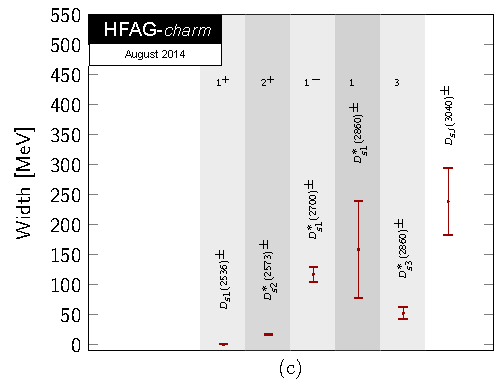
\includegraphics[width=0.45\textwidth]{./figures/charm/Dswidths}
\quad
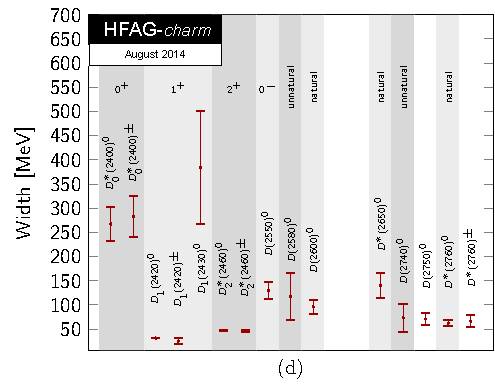
\includegraphics[width=0.45\textwidth]{./figures/charm/Dwidths}

\caption{\label{fig:charm:spect:1}  Summary of averaged masses for $D_{s}$ mesons are shown in subfigure (a) and for $D$ mesons in subfigure (b). The average widths for $D_{s}$ mesons are shown in subfigure (c) and for $D$ mesons in subfigure (d). The vertical shaded regions distinguish between different spin parity states.}
\end{centering}
\end{figure}

In the study of $B_{s}^{0}\to \overline{D}{}^{0}K^{-}\pi^{+}$ decays the LHCb collaboration searched excited excited  $D_{s}$ mesons~\cite{Aaij:2014xza}.  Previous measurements by \babar{}~\cite{Aubert:2009ah} and LHCb~\cite{Aaij:2012pc} indicated the existence of a strange-charm $D^{*}_{sJ}(2860)^{-}$ meson. The new measurement of LHCb showed with $10\sigma$ significance that this state is comprised of two different particles,  of spin 1 and and spin 3. This represents the first measurement of a heavy flavored spin-3 particle, and the first observation $B$ mesons decays to spin 3 particles.

The masses and widths of narrow ($\Gamma<50$~MeV) orbitally excited $D$ mesons (denoted $D^{\ast\ast}$), both neutral and charged, are well established. Measurements of broad states ($\Gamma\sim$ 200--400~MeV) are less abundant, as identifying the signal is more challenging. There is a slight discrepancy between the 
$D_0^\ast(2400)^0$ masses measured by the Belle\citep{Abe:2003zm} and  FOCUS\citep{Link:2003bd} experiments. No data exists yet for the $D_1(2430)^{\pm}$ state. Dalitz plot analyses of $B\to D^{(\ast)}\pi\pi$ decays strongly favor the assignments $0^+$ and $1^+$ for the spin-parity quantum numbers of the $D_0^\ast(2400)^0/D_0^\ast(2400)^\pm$ and $D_1(2430)^{0}$ states, respectively. The measured masses and widths, as well as the $J^P$ values, are in agreement with theoretical predictions based on potential models~\cite{PhysRevD.32.189, PhysRevLett.16.109, PhysRevD.43.1679, PhysRevLett.66.1130, PhysRevD.66.114004}. 


Table~\ref{table:charm:spect:3} and \ref{table:charm:spect:4} summarizes the branching fractions of $B$ mesons decays to excited $D$ and $D_{s}$ states, respectively. It can be noted that the branching fractions for $B$ mesons decaying to a narrow $D^{\ast\ast}$ state and a pion are similar for charged and neutral $B$ initial states, the branching fractions to a broad $D^{\ast\ast}$ state and $\pi^+$ are much larger for $B^+$ than for $B^0$. This may be due to the fact that color-suppressed amplitudes contribute only to the $B^+$ decay and not to the $B^0$ decay (for a theoretical discussion, see Ref.~\citep{PhysRevD.72.094010,Colangelo:2004vu}). Measurements of individual branching fractions of $D$ mesons are difficult due to the unknown fragmentation of $c\bar c \to D^{\ast\ast}$ or due to the unknown $B \to D^{\ast\ast} X$ branching fractions.

The discoveries of the $D_{s0}^\ast(2317)^{\pm}$ and $D_{s1}(2460)^{\pm}$ have triggered increased interest in properties of, and searches for, excited $D_s$ mesons (here generically denoted $D_s^{\ast\ast}$). While the masses and widths of $D_{s1}(2536)^{\pm}$ and $D_{s2}(2573)^{\pm}$ states are in relatively good agreement with potential model predictions, the masses of $D_{s0}^\ast(2317)^{\pm}$ and $D_{s1}(2460)^{\pm}$ states (and consequently their widths, less than around 5~MeV) are significantly lower than expected (see Ref.~\cite{PhysRevD.68.037502} for a discussion of $c\bar{s}$ models). Moreover, the mass splitting between these two states greatly exceeds that between the $D_{s1}(2536)^{\pm}$ and $D_{s2}(2573)^{\pm}$. These unexpected properties have led to interpretations of the $D_{s0}^\ast(2317)^{\pm}$ and $D_{s1}(2460)^{\pm}$ as exotic four-quark states~\cite{PhysRevD.68.054006,Lipkin:2003zk}.

While there are few measurements with respect to the $J^P$ values of $D_{s0}^\ast(2317)^{\pm}$ and $D_{s1}(2460)^{\pm}$, the available data favors $0^+$ and $1^+$, respectively. A molecule-like ($DK$) interpretation of the $D_{s0}^\ast(2317)^{\pm}$ and $D_{s1}(2460)^{\pm}$~\cite{Barnes:2003dj,Lipkin:2003zk} that can account for their low masses and isospin-breaking decay modes is tested by searching for charged and neutral isospin partners of these states; thus far such searches have yielded negative results. Therefore the subset of models that predict equal production rates for different charged states is nominally excluded. The molecular picture can also be tested by measuring the rates for the radiative processes $D_{s0}^\ast(2317)^{\pm}/D_{s1}(2460)^{\pm}\to D_s^{(\ast)}\gamma$ and comparing to theoretical predictions. The predicted rates, however, are below the sensitivity of current experiments. 

Another model successful in explaining the total widths and the $D_{s0}^\ast(2317)^{\pm}$ -- $D_{s1}(2460)^{\pm}$ mass splitting is based on the assumption that these states are chiral partners of the ground states $D_{s}^{+}$ and~$D_{s}^{*}$~\cite{PhysRevD.68.054024}. While some measured branching fraction ratios agree with predicted
values, further experimental tests with better sensitivity are needed to confirm or refute this scenario. A summary of the mass difference measurements is given in Table~\ref{table:charm:spect:5}.

In addition to the $D_{s0}^\ast(2317)^{\pm}$ and $D_{s1}(2460)^{\pm}$ states, other excited $D_s$ states may have been observed. SELEX has reported a $D_{sJ}(2632)^{\pm}$ candidate~\cite{Evdokimov:2004iy}, but this has not been confirmed by other experiments. Recently, Belle, \babar{} and LHCb have observed $D_{s1}(2700)^{\pm}$ which may be radial excitations of the $D_s^{\ast\pm}$. Equally the $D_{s1}(2860)^{\pm}$ measured by LHCb and $D_{sJ}(3040)^{\pm}$ measured by \babar{} could be excitations of $D_{s0}^\ast(2317)^{\pm}$ and $D_{s1}(2460)^{\pm}$ or $D_{s1}(2536)^{\pm}$, respectively (for a theoretical discussion, see Ref~\cite{Matsuki:2006rz}).

Table~\ref{table:charm:spect:6} summarizes measurements of the polarization amplitude $A_{D}$ (sometimes also referred as helicity parameter), which describe the initial polarization of the $D$ meson. In $D^{\ast\ast}$ meson decay the helicity distribution varies like $1 + A_{D}\cos^{2}\theta_{H}$, where $\theta_{H}$ is the angle in the $D^{\ast}$ rest frame between the two pions emitted by decay $D^{\ast\ast} \to D^{\ast}\pi$ and the $D^{\ast} \to D \pi$. The parameter is sensitive to possible S-wave contributions in the decay. In the case of an unpolarized $D$ meson decay decaying purely via D-wave the polarization amplitude is predicted to give $A_{D}=3$. 
Studies of the $D_{1}(2420)^{0}$ meson by the ZUES and \babar{} collaborations suggest that there is an S-wave admixture in the decay, which is  contrary to Heavy Quark Effective Theory calculations~\cite{Isgur:1989vq,Neubert:1993mb}.

\begin{table}[htb!]
\begin{adjustbox}{width=\textwidth,center}
{\setlength\tabcolsep{0pt}
	\begin{tabular}{cp{5pt}cp{5pt}cp{5pt}r@{}lp{5pt}r@{}lp{5pt}cp{5pt}c}
	\toprule
	\rowcolor{Gray} Resonance                 && $J^{P}$                   && Decay mode                                                         && \multicolumn{2}{c}{Mass [MeV$/c^{2}$]} && \multicolumn{2}{c}{Width [MeV]}      && \multicolumn{1}{c}{Measured by} && \multicolumn{1}{c}{Reference} 
	\\ \midrule
	\multirow{3}{*}{$D_{s0}^{*}(2317)^{\pm}$}	&&	\multirow{3}{*}{$0^{+}$}	&&	$D_{s}^{+}\pi^{0}$	&&$	2319$&$.6\pm0.2\pm1.4	$&&$	$&$	$&&	\babar{}	&&	\cite{Aubert:2006bk}          \\
		&&		&&	$D_{s}^{+}\pi^{0}$	&&$	2317$&$.3\pm0.4\pm0.8	$&&$	$&$	$&&	\babar{}	&&	\cite{Aubert:2003pe}          \\  \cmidrule{6-14}
		&&		&&		&\cellcolor{Gray}&$	\cellcolor{Gray}  2318$&\cellcolor{Gray}$.0 \pm 0.8	$&\cellcolor{Gray}&	\cellcolor{Gray}&\cellcolor{Gray}	&\cellcolor{Gray}&	\cellcolor{Gray} Our average	&\cellcolor{Gray}&	\\ \midrule
	%												
													
	\multirow{3}{*}{$D_{s1}(2460)^{\pm}$}	&&	\multirow{3}{*}{$1^{+}$}	&&	$D_{s}^{+}\pi^{0}\gamma, D_{s}^{+}\gamma, D_{s}^{+}\pi^{+}\pi^{-}$	&&$	2460$&$.1\pm0.2\pm0.8	$&&$	$&$	$&&	\babar{}	&&	\cite{Aubert:2006bk}          \\
		&&		&&	$D_{s}^{+}\pi^{0}\gamma$	&&$	2458$&${}\pm1.0\pm1.0	$&&$	$&$	$&&	\babar{}	&&	\cite{Aubert:2003pe}          \\ \cmidrule{6-14}
		&&		&&		&\cellcolor{Gray}&$	\cellcolor{Gray}  2459$&\cellcolor{Gray}$.6 \pm 0.7	$&\cellcolor{Gray}&	\cellcolor{Gray}&\cellcolor{Gray}	&\cellcolor{Gray}&	\cellcolor{Gray} Our average	&\cellcolor{Gray}&	\\ \midrule
	%												
	\multirow{11}{*}{$D_{s1}(2536)^{\pm}$}	&&	\multirow{11}{*}{$1^{+}$}	&&	$D^{*}{}^{+}K_{S}^{0}$	&&$	2535$&$.7\pm0.6\pm0.5	$&&$	$&$	$&&	D\O\ &&\cite{Abazov:2007wg}		\\
		&&		&&	$D^{*}{}^{+}K_{S}^{0}, D^{*}{}^{0}K^{+}$	&&$	2534$&$.78\pm0.31\pm0.40	$&&$	$&$	$&&	\babar{}	&&	\cite{Aubert:2007rva}         \\
		&&		&&	$D_{s}^{+}\pi^{+}\pi^{-}$	&&$	2534$&$.6\pm0.3\pm0.7	$&&$	$&$	$&&	\babar{}	&&	\cite{Aubert:2006bk}          \\
		&&		&&	$D^{*}{}^{+}K_{S}^{0}, D^{*}{}^{0}K^{+}$	&&$	2535$&$.0\pm0.6\pm1.0	$&&$	$&$	$&&	E687	&&	\cite{Frabetti:1993vv}        \\
		&&		&&	$D^{*}{}^{0}K^{+}$	&&$	2535$&$.3\pm0.2\pm0.5	$&&$	$&$	$&&	CLEO	&&	\cite{Alexander:1993nq}       \\
		&&		&&	$D^{*}{}^{+}K_{S}^{0}$	&&$	2534$&$.8\pm0.6\pm0.6	$&&$	$&$	$&&	CLEO	&&	\cite{Alexander:1993nq}       \\
		&&		&&	$D^{*}{}^{0}K^{+}$	&&$	2535$&$.2\pm0.5\pm1.5	$&&$	$&$	$&&	ARGUS	&&	\cite{Albrecht:1992zh}        \\
		&&		&&	$D^{*}{}^{+}K_{S}^{0}$	&&$	2535$&$.6\pm0.7\pm0.4	$&&$	$&$	$&&	CLEO	&&	\cite{Avery:1989ui}           \\
		&&		&&	$D^{*}{}^{+}K_{S}^{0}$	&&$	2535$&$.9\pm0.6\pm2.0	$&&$	$&$	$&&	ARGUS	&&	\cite{Albrecht:1989yi}        \\
		&&		&&	$D^{*}{}^{+}K_{S}^{0}$	&&$	$&$	$&&$	0$&$.92\pm0.03\pm0.04	$&&	\babar{}	&&	\cite{Lees:2011um}            \\ \cmidrule{6-14}
		&&		&&		&\cellcolor{Gray}&$	\cellcolor{Gray}2535$&\cellcolor{Gray}$.10 \pm 0.26	$&\cellcolor{Gray}&$	\cellcolor{Gray}0$&\cellcolor{Gray}$.92\pm0.05	$&\cellcolor{Gray}&	\cellcolor{Gray} Our average	&\cellcolor{Gray}&	\\ \midrule
													
	\multirow{5}{*}{$D_{s2}^{*}(2573)^{\pm}$}	&&	\multirow{5}{*}{$2^{+}$}	&&	$D^{0}K^{+}$	&&$	2568$&$.39\pm0.29\pm0.26	$&&$	16$&$.9\pm0.5\pm0.6	$&&	LHCb	&&	\cite{Aaij:2014baa}           \\
		&&		&&	$D^{+}K_{S}^{0}, D^{0}K^{+}$	&&$	2569$&$.4\pm1.6\pm0.5	$&&$	12$&$.1\pm4.5\pm1.6	$&&	LHCb	&&	\cite{Aaij:2011ju}            \\
		&&		&&	$D^{+}K_{S}^{0}, D^{0}K^{+}$	&&$	2572$&$.2\pm0.3\pm1.0	$&&$	27$&$.1\pm0.6\pm5.6	$&&	\babar{}	&&	\cite{Aubert:2006mh}          \\
		&&		&&	$D^{0}K^{+}$	&&$	2574$&$.25\pm3.3\pm1.6	$&&$	10$&$.4\pm8.3\pm3.0	$&&	ARGUS	&&	\cite{Albrecht:1995qx}        \\
		&&		&&	$D^{0}K^{+}$	&&$	2573$&$.2 _{-1.6}^{+1.7}\pm0.9	$&&$	16$&${}_{-4}^{+5}\pm3	$&&	CLEO	&&	\cite{Kubota:1994gn}          \\ \cmidrule{6-14}
		&&		&&		&\cellcolor{Gray}&$	\cellcolor{Gray}2569$&\cellcolor{Gray}$.08 \pm 0.35	$&\cellcolor{Gray}&$	\cellcolor{Gray} 16$&\cellcolor{Gray}$.9 \pm 0.8	$&\cellcolor{Gray}&	\cellcolor{Gray}Our average	&\cellcolor{Gray}&	\\ \midrule
													
	\multirow{4}{*}{$D_{s1}^{*}(2700)^{\pm}$}	&&	\multirow{4}{*}{$1^{-}$}	&&	$D^{*}{}^{+}K_{S}^{0}, D^{*}{}^{0}K^{+}$	&&$	2709$&$.2\pm1.9\pm4.5	$&&$	115$&$.8\pm7.3\pm12.1	$&&	LHCb	&&	\cite{Aaij:2012pc}            \\
		&&		&&	$DK, D^{*}K$	&&$	2710$&${}\pm 2 _{-7}^{+12}	$&&$	149$&${}\pm7 _{-52}^{+39}	$&&	\babar{}	&&	\cite{Aubert:2009ah}          \\
		&&		&&	$D^{0}K^{+}$	&&$	2708$&${}\pm9 _{-10}^{+11}	$&&$	108$&${}\pm2. _{-31}^{+36}	$&&	Belle	&&	\cite{Brodzicka:2007aa}       \\ \cmidrule{6-14}
		&&		&&		&\cellcolor{Gray}&$	\cellcolor{Gray} 2709$&\cellcolor{Gray}$.2 \pm 4.2	$&\cellcolor{Gray}&$	\cellcolor{Gray} 117$&\cellcolor{Gray}$.2 \pm 12.5	$&\cellcolor{Gray}&	\cellcolor{Gray} Our average	&\cellcolor{Gray}&	\\ \midrule
	%												
	\multirow{1}{*}{$D_{s1}^{*}(2860)^{\pm}$}	&&	\multirow{1}{*}{1}	&&	$ D^{0}K^{+}$	&\cellcolor{LightGray} &$	\cellcolor{LightGray} 2859$&\cellcolor{LightGray}${}\pm12\pm24	$&\cellcolor{LightGray}&$	\cellcolor{LightGray} 159$&\cellcolor{LightGray}${}\pm23\pm77	$&\cellcolor{LightGray}&	\cellcolor{LightGray} LHCb	&\cellcolor{LightGray}&	\cite{Aaij:2014xza}           \\ \midrule
	%												
	\multirow{1}{*}{$D_{s3}^{*}(2860)^{\pm}$}	&&	\multirow{1}{*}{3}	&&	$ D^{0}K^{+}$	&\cellcolor{LightGray}&$	\cellcolor{LightGray} 2860$&\cellcolor{LightGray}$.5\pm2.6\pm6.5	$&\cellcolor{LightGray}&$	\cellcolor{LightGray} 53$&\cellcolor{LightGray}${}\pm7\pm7	$&\cellcolor{LightGray}&	\cellcolor{LightGray} LHCb	&\cellcolor{LightGray}&	\cite{Aaij:2014xza}           \\ \midrule
	%												
	\multirow{1}{*}{$D_{sJ}(3040)^{\pm}$}	&&	\multirow{1}{*}{}	&&	$D^{*}K$	&\cellcolor{LightGray}&$	\cellcolor{LightGray} 3044$&\cellcolor{LightGray}${}\pm8 _{-5}^{+30}	$&\cellcolor{LightGray}&$	\cellcolor{LightGray}239$&\cellcolor{LightGray}${}\pm35 _{-42}^{+46}	$&\cellcolor{LightGray}&	\cellcolor{LightGray} \babar{}	&\cellcolor{LightGray}&	\cite{Aubert:2009ah}          \\ \bottomrule
\end{tabular}
}
\end{adjustbox}

\caption{\label{table:charm:spect:1} Summary of recent measurements of mass and width for different excited $D_{s}$ mesons. The column $J^{P}$ list the most significant assignment of spin and parity. If possible an average mass or width is calculated.}
\end{table} 

\begin{table}[htb!]
%\badj
\begin{tabular}{cccS[parse-numbers=false,separate-uncertainty=true,table-format=5.11]S[parse-numbers=false,separate-uncertainty=true,table-format=3.11]cc}
\toprule
\rowcolor{Gray}  Resonance&$J^{P}$ & Decay mode &  \multicolumn{1}{c}{Mass [\si{\MeV$/c^{2}$}]} &  \multicolumn{1}{c}{Width [\si{\MeV}]} &  \multicolumn{1}{c}{Measured by} &  \multicolumn{1}{c}{Reference}
 \\ \midrule
 %D*0(2400)0 	
\multirow{4}{*}{$D_{0}^{*}(2400)^{0}$} &  \multirow{4}{*}{$0^{+}$} &$D^{+}\pi^{-}$ & 2297.\pm8\pm20 & 273.\pm12\pm48 & \babar{} &\cite{Aubert:2009wg}\\
												& &$D^{+}\pi^{-}$ &2308.\pm17\pm32& 276.\pm21\pm63& Belle &\cite{Abe:2003zm}\\
												& &$D^{+}\pi^{-}$ & 2407. \pm 21 \pm 35& 240. \pm55 \pm 59& Focus &\cite{Link:2003bd}\\ \cmidrule{4-6}
												& & &\cellcolor{Gray}  2318.2 \pm 16.9&\cellcolor{Gray}  267.4 \pm 35.6&\cellcolor{Gray}  Our average &\\ \midrule
%
%D*0(2400)+-
\multirow{1}{*}{$D_{0}^{*}(2400)^{\pm}$} & \multirow{1}{*}{$0^{+}$} &$D^{0}\pi^{+}$ & \cellcolor{LightGray}2403. \pm 14 \pm35 & \cellcolor{LightGray}283 \pm24 \pm34 &\cellcolor{LightGray} Focus($m$ \& $\Gamma$) + Belle($J^{P}$) &\cite{Link:2003bd} + \cite{Kuzmin:2006mw}\\ \midrule
%
%D1(2420)0 	
\multirow{11}{*}{$D_{1}^{}(2420)^{0}$} &  \multirow{11}{*}{$1^{+}$} &$D^{*+}\pi^{-}$ & 2419.6\pm0.1\pm0.7 &35.2\pm0.4\pm0.9& LHCb & \cite{Aaij:2013sza}\\
												&  &$D^{*+}\pi^{-}$ & 2423.1 \pm 1.5 ^{+0.4}_{-1.0} &38.8\pm5^{+1.9}_{-5.4}& Zeus & \cite{Abramowicz:2012ys}\\
												& &$D^{*+}\pi^{-}$ &2420.1 \pm0.1 \pm0.8 &31.4\pm0.5\pm1.3 & \babar{}& \cite{delAmoSanchez:2010vq}\\
												& &$D^{*+}\pi^{-}$ & &20.0\pm1.7\pm1.3 & CDF& \cite{Abulencia:2005ry}\\
												& &$D^{0}\pi^{+}\pi^{-}$ &2426. \pm3 \pm1&24.\pm7\pm8 &Belle & \cite{Abe:2004sm}\\
												& &$D^{*+}\pi^{-}$ &2421.4 \pm1.5 \pm 0.9&23.7\pm2.7\pm4.0& Belle&\cite{Abe:2003zm} \\
												& &$D^{*+}\pi^{-}$ &2421.^{+1}_{-2}\pm2&20.^{+6}_{-5}{}^{+3}_{-3}& CLEO&\cite{Avery:1994yc} \\												
												& &$D^{*+}\pi^{-}$ &2422. \pm2 \pm2&15.\pm8\pm4& E687&\cite{Frabetti:1993vv} \\																		
												& &$D^{*+}\pi^{-}$ &2428.\pm3\pm2&23.^{+8}_{-6}{}^{+10}_{-4}& CLEO& \cite{Avery:1989ui}\\	
												& &$D^{*+}\pi^{-}$ &2414.\pm2\pm5&13.\pm6^{+10}_{-5}& Argus&\cite{Albrecht:1989pa} \\	 
												& &$D^{*+}\pi^{-}$ &2428. \pm 8 \pm5&58. \pm14 \pm10& TPS&\cite{Anjos:1988uf} \\ \cmidrule{4-6}											
												& &&\cellcolor{Gray}  2420.5 \pm 0.5 &\cellcolor{Gray} 31.7 \pm 0.7  &\cellcolor{Gray}  Our average &\\ \midrule
%D1(2420)+- 	 	
\multirow{5}{*}{$D_{1}^{}(2420)^{\pm}$} &  \multirow{5}{*}{$1^{+}$} &$D^{*0}\pi^{+}$ &2421.9\pm4.7^{+3.4}_{-1.2} &  & Zeus &\cite{Abramowicz:2012ys}\\
												& &$D^{+}\pi^{-}\pi^{+}$ &2421.\pm2\pm1& 21.\pm5\pm8& Belle &\cite{Abe:2004sm}\\
												& &$D^{*0}\pi^{+}$ & 2425.\pm2\pm2& 26.^{+8}_{-7}\pm4& CLEO &\cite{Bergfeld:1994af}\\
												& &$D^{*0}\pi^{+}$ & 2443. \pm7\pm5& 41.\pm19\pm8& TPS &\cite{Anjos:1988uf}\\ \cmidrule{4-6}	
												& &&\cellcolor{Gray}   2423.2 \pm 1.6 &\cellcolor{Gray}  25.2 \pm 6.0  &\cellcolor{Gray}   Our average &\\ \midrule
%D*1(2430)0
\multirow{1}{*}{$D_{1}(2430)^{0}$} & \multirow{1}{*}{$1^{+}$} &$D^{*+}\pi^{-}$ & \cellcolor{LightGray}2427.\pm26\pm25&\cellcolor{LightGray} 384.^{+107}_{-75}\pm74 &\cellcolor{LightGray} Belle &\cite{Abe:2003zm} \\ \midrule
%D*2(2460)0 	
\multirow{14}{*}{$D_{2}^{*}(2460)^{0}$} &  \multirow{14}{*}{$2^{+}$} & $D^{*+}\pi^{-}$ & 2460.4\pm0.4\pm1.2& 43.2\pm1.2\pm3.0&LHCb&\cite{Aaij:2013sza} \\
												& & $D^{+}\pi^{-}$ & 2460.4\pm0.1\pm0.1& 45.6\pm0.4\pm1.1&LHCb&\cite{Aaij:2013sza} \\
												& &$D^{*+}\pi^{-}$, $D^{+}\pi^{-}$ & 2462.5\pm2.4^{+1.3}_{-1.1}& 46.6\pm8.1^{+5.9}_{-3.8}& Zeus & \cite{Abramowicz:2012ys}\\
												& &$D^{+}\pi^{-}$ & 2462.2\pm0.1\pm0.8& 50.5\pm0.6\pm0.7& \babar{}& \cite{delAmoSanchez:2010vq}\\
												& &$D^{+}\pi^{-}$ & 2460.4\pm1.2\pm2.2& 41.8\pm2.5\pm2.9& \babar{}& \cite{Aubert:2009wg}\\
												& &$D^{+}\pi^{-}$ & &49.2\pm2.3\pm1.3& CDF& \cite{Abulencia:2005ry}\\												
												& &$D^{+}\pi^{-}$ & 2461.6\pm2.1\pm3.3& 45.6\pm4.4\pm6.7&Belle & \cite{Abe:2003zm}\\
												& &$D^{+}\pi^{-}$ & 2464.5\pm1.1\pm1.9& 38.7\pm5.3\pm2.9& Focus&\cite{Link:2003bd} \\
												& &$D^{+}\pi^{-}$ & 2465.\pm3\pm3& 28.^{+8}_{-7}\pm6& CLEO&\cite{Avery:1994yc} \\												
												& &$D^{+}\pi^{-}$ & 2453.\pm3\pm2& 25.\pm10\pm5& E687&\cite{Frabetti:1993vv} \\																	
												& &$D^{*+}\pi^{-}$ & 2461.\pm3\pm1& 20.^{+9}_{-12}{}^{+9}_{-10}& CLEO& \cite{Avery:1989ui}\\	
												& &$D^{+}\pi^{-}$ & 2455.\pm3\pm5& 15.^{+13}_{-10}{}^{+5}_{-10}& Argus&\cite{Albrecht:1988dj} \\												
												& &$D^{+}\pi^{-}$ & 2459.\pm3\pm2& 20.\pm10\pm5& TPS&\cite{Anjos:1988uf} \\	 \cmidrule{4-6}															
												& &&\cellcolor{Gray}  2460.47 \pm 0.14 &\cellcolor{Gray} 47.7 \pm 0.7  &\cellcolor{Gray}  Our average &\\ \midrule
%D*2(2460)+- 
\multirow{9}{*}{$D_{2}^{*}(2460)^{\pm}$} &  \multirow{9}{*}{$2^{+}$} & $D^{0}\pi^{+}$ & 2463.1\pm0.2\pm0.6 & 48.6\pm1.3\pm1.9& LHCb &\cite{Aaij:2013sza} \\ 
												&&$D^{*0}\pi^{+}$, $D^{0}\pi^{+}$ & 2460.6\pm4.4^{+3.6}_{-0.8}& & Zeus & \cite{Abramowicz:2012ys}\\
												& &$D^{0}\pi^{+}$ & 2465.4\pm0.2\pm1.1& & \babar{}& \cite{delAmoSanchez:2010vq}\\
												& &$D^{0}\pi^{+}$ & 2465.7\pm1.8^{+1.4}_{-4.8}& 49.7\pm3.8\pm6.4& Belle& \cite{Kuzmin:2006mw}\\
												& &$D^{0}\pi^{+}$ & 2467.6\pm1.5\pm0.8 & 34.1\pm6.5\pm4.2& Focus& \cite{Link:2003bd}\\
												& &$D^{0}\pi^{+}$ & 2463.\pm3\pm3& 27.^{+11}_{-8}\pm5& CLEO& \cite{Bergfeld:1994af}\\												
												& &$D^{0}\pi^{+}$ & 2453.\pm3\pm2& 23.\pm9\pm5&E687 & \cite{Frabetti:1993vv}\\
												& &$D^{0}\pi^{+}$ &2469.\pm4\pm6 & & Argus&\cite{Albrecht:1988xx} \\  \cmidrule{4-6}	
												& &&\cellcolor{Gray} 2463.8 \pm 0.5 &\cellcolor{Gray}45.9 \pm 2.0  &\cellcolor{Gray} Our average &\\ \midrule
%D(2550)^{0}
\multirow{1}{*}{$D(2550)^{0}$} & \multirow{1}{*}{$0^{-}$} &$D^{*+}\pi^{-}$ & \cellcolor{LightGray}2539.4\pm4.5\pm6.8& \cellcolor{LightGray}130.\pm12\pm13 &\cellcolor{LightGray} \babar{} &\cite{delAmoSanchez:2010vq} \\ \midrule	
%D(2550)^{0}
\multirow{1}{*}{$D(2580)^{0}$} & \multirow{1}{*}{Unnatural} &$D^{*+}\pi^{-}$ & \cellcolor{LightGray}2579.5\pm3.4\pm5.5&\cellcolor{LightGray} 117.5\pm17.8\pm46.0 &\cellcolor{LightGray} LHCb &\cite{Aaij:2013sza} \\ \midrule	
%D(2550)^{0}
\multirow{1}{*}{$D(2600)^{0}$} & \multirow{1}{*}{Natural} &$D^{+}\pi^{-}$ & \cellcolor{LightGray}2608.7\pm2.4\pm2.5&\cellcolor{LightGray} 93.\pm6\pm13 &\cellcolor{LightGray} \babar{} &\cite{delAmoSanchez:2010vq} \\ \midrule	
%D(2550)^{0}
\multirow{1}{*}{$D(2600)^{\pm}$} & \multirow{1}{*}{Natural} &$D^{0}\pi^{+}$ & \cellcolor{LightGray}2621.3\pm3.7\pm4.2&\cellcolor{LightGray}  &\cellcolor{LightGray} \babar{} &\cite{delAmoSanchez:2010vq} \\ \midrule						
%D(2550)^{0}
\multirow{1}{*}{$D^{*}(2640)^{\pm}$} & \multirow{1}{*}{$1^{-}$} &$D^{*+}\pi^{+}\pi^{-}$ & \cellcolor{LightGray}2637.\pm2\pm6&\cellcolor{LightGray}  &\cellcolor{LightGray} Delphi &\cite{Abreu:1998vk} \\ \midrule						
%D(2550)^{0}
\multirow{1}{*}{$D^{*}(2650)^{0}$} & \multirow{1}{*}{Natural} &$D^{*+}\pi^{-}$ & \cellcolor{LightGray}2649.2\pm3.5\pm3.5&\cellcolor{LightGray}140.2\pm17.1\pm18.6  &\cellcolor{LightGray} LHCb &\cite{Aaij:2013sza} \\ \midrule		
%
\multirow{1}{*}{$D(2740)^{0}$} & \multirow{1}{*}{Unnatural} &$D^{*+}\pi^{-}$ & \cellcolor{LightGray} 2737.0\pm3.5\pm11.2& \cellcolor{LightGray} 73.2\pm13.4\pm25.0 & \cellcolor{LightGray} LHCb &\cite{Aaij:2013sza} \\ \midrule
%D(2550)^{0}
\multirow{1}{*}{$D(2750)^{0}$} & \multirow{1}{*}{} &$D^{*+}\pi^{-}$ & \cellcolor{LightGray} 2752.4\pm1.7\pm2.7& \cellcolor{LightGray} 71.\pm6\pm11 & \cellcolor{LightGray} \babar{} &\cite{delAmoSanchez:2010vq} \\ \midrule	
%D(2550)^{0}
\multirow{4}{*}{$D^{*}(2760)^{0}$} & \multirow{4}{*}{Natural} &$D^{*+}\pi^{-}$ & 2761.1\pm5.1\pm6.5&74.4\pm3.4\pm37.0  & LHCb &\cite{Aaij:2013sza} \\ 
											&&$D^{+}\pi^{-}$ & 2760.1\pm1.1\pm3.7&74.4\pm3.4\pm19.1 & LHCb &\cite{Aaij:2013sza} \\ 		
											&&$D^{+}\pi^{-}$ & 2763.3\pm2.3\pm2.3& 60.9\pm5.1\pm3.6& \babar{}& \cite{delAmoSanchez:2010vq}\\  \cmidrule{4-6}
											&&&\cellcolor{Gray} 2761.9 \pm 2.4 &\cellcolor{Gray} 62.5 \pm 5.9&\cellcolor{Gray}  Our average & \\ \midrule
%
\multirow{3}{*}{$D^{*}(2760)^{\pm}$} & \multirow{1}{*}{}&$D^{0}\pi^{+}$ & 2771.7\pm1.7\pm3.8&66.7\pm6.6\pm10.5 & LHCb &\cite{Aaij:2013sza} \\ 	 							 
										&&$D^{0}\pi^{+}$ &2769.7\pm3.8\pm1.5&  &  \babar{} &\cite{delAmoSanchez:2010vq} \\ \cmidrule{4-6}
											&&&\cellcolor{Gray} 2770.7 \pm 2.9 &\cellcolor{Gray} 66.7\pm12.4&\cellcolor{Gray}  Our average & \\ \bottomrule
\end{tabular}
%\eadj

\caption{\label{tabel:charm:spect:2} Summary of recent measurements of mass and width for different excited $D$ mesons. The column $J^{P}$ list the most significant assignment of spin and parity. If possible an average mass or width is calculated.}
\end{table} 


\begin{table}[htb!]
\begin{center}
\begin{tabular}{ccS[parse-numbers=false,separate-uncertainty=true,table-format=5.11]cc}
\toprule
\rowcolor{Gray} Resonance&Decay &\multicolumn{1}{c}{$\mathcal{B}r[10^{-4}]$} &  \multicolumn{1}{c}{Measured by} &  \multicolumn{1}{c}{Reference}
 \\ \midrule
\multirow{3}{*}{$D_{0}^{*}(2400)^{0}$} & \multirow{3}{*}{$B^{-}\to D_{0}^{*}(2400)^{0}(\to D^{+}\pi^{-})\pi^{-}$} & 6.1\pm0.6\pm1.8 & Belle &\cite{Abe:2003zm}\\ 
																		& & 6.8\pm0.3\pm2.0 & \babar{} &\cite{Aubert:2009wg}\\  \cmidrule{3-4}
																	& &\cellcolor{Gray}6.4\pm 1.4  &\cellcolor{Gray}  Our average &\\ \midrule
%
\multirow{1}{*}{$D_{0}^{*}(2400)^{\pm}$} & \multirow{1}{*}{$\overline{B}{}^{0}\to D_{0}^{*}(2400)^{+}(\to D^{0}\pi^{-})\pi^{-}$} &\cellcolor{LightGray} 0.60\pm0.13\pm0.27 &\cellcolor{LightGray} Belle &\cite{Kuzmin:2006mw}\\	\midrule		
%
\multirow{2}{*}{$D_{1}^{}(2420)^{0}$} & \multirow{1}{*}{$B^{-}\to D_{1}^{}(2420)^{0}(\to D^{*+}\pi^{-})\pi^{-}$} &\cellcolor{LightGray} 6.8\pm0.7\pm1.3 &\cellcolor{LightGray} Belle &\cite{Abe:2003zm}\\	\cmidrule{2-4}
& \multirow{1}{*}{$B^{-}\to D_{1}^{}(2420)^{0}(\to D^{0}\pi^{+}\pi^{-})\pi^{-}$} &\cellcolor{LightGray} 1.85\pm0.29\pm0.27\pm0.41 &\cellcolor{LightGray} Belle &\cite{Abe:2004sm}\\	\midrule					
%				
\multirow{1}{*}{$D_{1}^{}(2420)^{\pm}$} & \multirow{1}{*}{$\overline{B}{}^{0}\to D_{1}(2420)^{+}(\to D^{+}\pi^{-}\pi^{+})\pi^{-}$} &\cellcolor{LightGray} 0.89\pm0.15\pm0.22 &\cellcolor{LightGray} Belle &\cite{Abe:2004sm}\\ \midrule
%
\multirow{1}{*}{$D_{1}(2430)^{0}$} &$B^{-}\to D_{1}(2430)^{0}(\to D^{*+}\pi^{-})\pi^{-}$ & \cellcolor{LightGray}5.0\pm0.4\pm1.08 &\cellcolor{LightGray} Belle &\cite{Abe:2003zm} \\ \midrule
%%D*2(2460)0 	
\multirow{4}{*}[-5pt]{$D_{2}^{*}(2460)^{0}$}  & \multirow{3}{*}{$B^{-}\to D_{2}^{*}(2460)^{0}(\to D^{+}\pi^{-})\pi^{-}$} &3.4\pm0.3\pm0.7 &Belle &\cite{Abe:2003zm}\\ 
																 & & 3.5\pm0.2\pm0.5 & \babar{} &\cite{Aubert:2009wg}\\ \cmidrule{3-4}
 																	& &\cellcolor{Gray} 3.5 \pm 0.3 &\cellcolor{Gray}  Our average &\\ \cmidrule{2-4}
& \multirow{1}{*}{$B^{-}\to D_{2}^{*}(2460)^{0}(\to D^{*+}\pi^{-})\pi^{-}$} &\cellcolor{LightGray} 1.8\pm0.3\pm0.4 &\cellcolor{LightGray} Belle &\cite{Abe:2003zm}\\ \midrule
%
\multirow{1}{*}{$D_{2}^{*}(2460)^{\pm}$} & \multirow{1}{*}{$\overline{B}{}^{0}\to D_{2}^{*}(2460)^{+}(\to D^{0}\pi^{-})\pi^{-}$} &\cellcolor{LightGray} 2.15\pm0.17\pm0.31 &\cellcolor{LightGray} Belle &\cite{Kuzmin:2006mw}\\	\bottomrule	
\end{tabular}
\caption{\label{table:charm:spect:3} Summary of branching fraction of $B$ mesons decays to excited $D$ mesons.}
\end{center}
\end{table} 

\begin{table}[htb!]
\begin{center}
\begin{tabular}{ccS[parse-numbers=false,separate-uncertainty=true,table-format=5.11]cc}
\toprule
\rowcolor{Gray} Resonance&Decay &\multicolumn{1}{c}{$\mathcal{B}r[10^{-4}]$} &  \multicolumn{1}{c}{Measured by} &  \multicolumn{1}{c}{Reference}
 \\ \midrule
\multirow{4}{*}[-5pt]{$D_{s0}^{*}(2317)^{\pm}$} & \multirow{3}{*}{$B^{0}\to D_{s0}^{*}(2317)^{+}(\to D^{+}_{s}\pi^{0})D^{-}$} & 8.6^{+3.3}_{-2.6}\pm2.6 & Belle &\cite{Krokovny:2003zq}\\ 
																		& & 18.\pm 4{}^{+6.7}_{-5} & \babar{} &\cite{Aubert:2004pw}\\  \cmidrule{3-4}
																	& &\cellcolor{Gray}10.8 \pm 3.4  &\cellcolor{Gray}  Our average &\\ \cmidrule{2-4}
							&\multirow{1}{*}{$B^{0}\to D_{s0}^{*}(2317)^{+}(\to D^{+}_{s}\pi^{0})K^{-}$} &\cellcolor{LightGray}  0.53^{+0.15}_{-0.13}\pm0.16&\cellcolor{LightGray}  Belle & \cite{Abe:2004wz} \\ \midrule
																	
%
\multirow{9}{*}[-5pt]{$D_{s1}(2460)^{\pm}$} & \multirow{3}{*}{$B^{0}\to D_{s1}(2460)^{+}(\to D^{*+}_{s}\pi^{0})D^{-}$} & 22.7^{+7.3}_{-6.2}\pm6.8 & Belle &\cite{Krokovny:2003zq}\\ 
																		& & 28.\pm 8{}^{+11.2}_{-7.8} & \babar{} &\cite{Aubert:2004pw}\\  \cmidrule{3-4}
																	& &\cellcolor{Gray}24.7 \pm 7.6  &\cellcolor{Gray}  Our average &\\ \cmidrule{2-4}
%
& \multirow{3}{*}{$B^{0}\to D_{s1}(2460)^{\pm}(\to D^{*+}_{s}\gamma)D^{-}$} & 8.2^{+2.2}_{-1.9}\pm2.5 & Belle &\cite{Krokovny:2003zq}\\ 
																		& & 8.\pm 2{}^{+3.2}_{-2.3} & \babar{} &\cite{Aubert:2004pw}\\  \cmidrule{3-4}
																	& &\cellcolor{Gray}8.1 \pm 2.3 &\cellcolor{Gray}  Our average &\\ \cmidrule{2-4}
							& $D_{s1}(2460)^{+}\to D^{*-}_{s}\pi^{0}$&\cellcolor{LightGray} (56.\pm13\pm9)\%&\cellcolor{LightGray} \babar{}&\cite{Aubert:2006nm} \\ \cmidrule{2-4}								
							& $D_{s1}(2460)^{+}\to D^{*-}_{s}\gamma$&\cellcolor{LightGray} (16.\pm4\pm3)\%&\cellcolor{LightGray} \babar{}&\cite{Aubert:2006nm} \\ \midrule					
%
								 & \multirow{1}{*}{$B^{0}\to D_{s1}(2536)^{+}(\to D^{*0}K^{+})D^{-}$} &\cellcolor{LightGray} 1.71\pm0.48\pm0.32 &\cellcolor{LightGray} \babar{} &\cite{Aubert:2007rva}\\ \cmidrule{2-4}
								& \multirow{1}{*}{$B^{0}\to D_{s1}(2536)^{+}(\to D^{*+}K^{0})D^{-}$} &\cellcolor{LightGray} 2.61\pm1.03\pm0.31 &\cellcolor{LightGray} \babar{} &\cite{Aubert:2007rva}\\ \cmidrule{2-4}
							 &\multirow{1}{*}{$B^{0}\to D_{s1}(2536)^{+}(\to D^{*0}K^{+})D^{*-}$} &\cellcolor{LightGray} 3.32\pm0.88\pm0.66 &\cellcolor{LightGray} \babar{} &\cite{Aubert:2007rva}\\ \cmidrule{2-4}
\multirow{2}{*}{$D_{s1}(2536)^{\pm}$}&\multirow{1}{*}{$B^{0}\to D_{s1}(2536)^{+}(\to D^{*+}K^{0})D^{*-}$} &\cellcolor{LightGray} 5.00\pm1.51\pm0.67 &\cellcolor{LightGray} \babar{} &\cite{Aubert:2007rva}\\ \cmidrule{2-4}
							 &\multirow{1}{*}{$B^{+}\to D_{s1}(2536)^{+}(\to D^{*0}K^{+})\overline{D}^{0}$} &\cellcolor{LightGray} 2.16\pm0.52\pm0.45 &\cellcolor{LightGray} \babar{} &\cite{Aubert:2007rva}\\ \cmidrule{2-4}
							&\multirow{1}{*}{$B^{+}\to D_{s1}(2536)^{+}(\to D^{*+}K^{0})\overline{D}^{0}$} &\cellcolor{LightGray} 2.30\pm0.98\pm0.43 &\cellcolor{LightGray} \babar{} &\cite{Aubert:2007rva}\\ \cmidrule{2-4}
							 &\multirow{1}{*}{$B^{+}\to D_{s1}(2536)^{+}(\to D^{*0}K^{+})\overline{D}^{*0}$} &\cellcolor{LightGray} 5.46\pm1.17\pm1.04 &\cellcolor{LightGray} \babar{} &\cite{Aubert:2007rva}\\ \cmidrule{2-4}
							&\multirow{1}{*}{$B^{+}\to D_{s1}(2536)^{+}(\to D^{*+}K^{0})\overline{D}^{*0}$}  &\cellcolor{LightGray} 3.92\pm2.46\pm0.83 &\cellcolor{LightGray} \babar{} &\cite{Aubert:2007rva}\\ \midrule
%
\multirow{1}{*}{$D_{s1}(2700)^{\pm}$} & \multirow{1}{*}{$B^{+}\to D_{s1}(2700)^{+}(\to D^{0}K^{+})\overline{D}{}^{0}$} &\cellcolor{LightGray}  11.3\pm2.2{}^{+1.4}_{-2.8} &\cellcolor{LightGray}  Belle &\cite{Brodzicka:2007aa}\\ \bottomrule
\end{tabular}
\caption{\label{table:charm:spect:4} Summary of branching fraction of $B$ mesons decays to excited $D_{s}$ mesons.}
\end{center}
\end{table} 


\begin{table}[htb!]
\begin{center}
{\setlength\tabcolsep{0pt}
	\begin{tabular}{cp{5pt}cp{5pt}r@{}lp{5pt}cp{5pt}c}
		\toprule
		\rowcolor{Gray}  Resonance                      &   & Relative to                                  && \multicolumn{2}{c}{$\Delta m$ [MeV$/c^{2}$]} & & \multicolumn{1}{c}{Measured by} && \multicolumn{1}{c}{Reference} 
		\\ \midrule
		%D*0(2400)0 	
		\multirow{3}{*}{$D_{1}^{*}(2420)^{0}$}          &   & \multirow{3}{*}{$D^{*+}$}                    &                       & $	410$                       & $.2\pm2.1\pm0.9	$                              &                       & Zeus                          &                       & \cite{Chekanov:2008ac}  \\
		                                                &   &                                              &                       & $	411$                       & $.7\pm0.7\pm0.4	$                              &                       & CDF                           &                       & \cite{Abulencia:2005ry} \\ \cmidrule{4-9}
		                                                &   &                                              & \cellcolor{Gray}      & \cellcolor{Gray} $411$       & \cellcolor{Gray}$.5 \pm 0.8	$                  & \cellcolor{Gray}      & \cellcolor{Gray}  Our average & \cellcolor{Gray}      &                         \\ \midrule
		%								
													
		\multirow{1}{*}{$D_{1}^{}(2420)^{\pm}$}         &   & \multirow{1}{*}{$D_{1}^{*}(2420)^{0}$}       & \cellcolor{LightGray} & $	\cellcolor{LightGray}4$    & \cellcolor{LightGray}${}^{+2}_{-3}\pm3	$       & \cellcolor{LightGray} & \cellcolor{LightGray} CLEO    & \cellcolor{LightGray} & \cite{Bergfeld:1994af}  \\ \midrule
													
		\multirow{2}{*}{$D_{2}^{*}(2460)^{0}$}          &   & $D^{+}$                                      & \cellcolor{LightGray} & $	\cellcolor{LightGray}593$  & \cellcolor{LightGray}$.9\pm0.6\pm0.5	$         & \cellcolor{LightGray} & \cellcolor{LightGray}CDF      & \cellcolor{LightGray} & \cite{Abulencia:2005ry} \\  \cmidrule{3-9}
		                                                &   & $D^{*+}$                                     & \cellcolor{LightGray} & $	\cellcolor{LightGray} 458$ & \cellcolor{LightGray}$.8\pm3.7^{+1.2}_{-1.3}	$ & \cellcolor{LightGray} & \cellcolor{LightGray} Zeus    & \cellcolor{LightGray} & \cite{Chekanov:2008ac}  \\ \midrule
		%D*2(2460)+-								
		\multirow{4}{*}[-2pt]{$D_{2}^{*}(2460)^{\pm}$}  &   & \multirow{4}{*}[-2pt]{$D_{2}^{*}(2460)^{0}$} &                       & $	3$                         & $.1\pm1.9\pm0.9	$                              &                       & Focus                         &                       & \cite{Link:2003bd}      \\
		                                                &   &                                              &                       & $-2$                         & ${}\pm4\pm4	$                                  &                       & CLEO                          &                       & \cite{Bergfeld:1994af}  \\
		                                                &   &                                              &                       & $	14$                        & ${}\pm5\pm8	$                                  &                       & ARGUS                         &                       & \cite{Albrecht:1989gb}  \\ \cmidrule{4-9}
		                                                &   &                                              & \cellcolor{Gray}      & $	\cellcolor{Gray}  3$       & \cellcolor{Gray}$.0 \pm 1.9	$                  & \cellcolor{Gray}      & \cellcolor{Gray} Our average  & \cellcolor{Gray}      &                         \\ \midrule
		%D(2550)^{0}								
													
													
		\multirow{4}{*}[-2pt]{$D_{s0}^{*}(2317)^{\pm}$} &   & \multirow{4}{*}[-2pt]{$D_{s}^{\pm}$}         &                       & $	348$                       & $.7\pm0.5\pm0.7	$                              &                       & Belle                         &                       & \cite{Abe:2003jk}       \\
		                                                &   &                                              &                       & $	350$                       & $.0\pm1.2\pm1.0	$                              &                       & CLEO                          &                       & \cite{Besson:2003cp}    \\
		                                                &   &                                              &                       & $	351$                       & $.3\pm2.1\pm1.9	$                              &                       & Belle                         &                       & \cite{Krokovny:2003zq}  \\ \cmidrule{4-9}
		                                                &   &                                              & \cellcolor{Gray}      & $	\cellcolor{Gray}  349$     & \cellcolor{Gray}$.2 \pm 0.7	$                  & \cellcolor{Gray}      & \cellcolor{Gray} Our average  & \cellcolor{Gray}      &                         \\ \midrule
		\multirow{7}{*}[-5pt]{$D_{s1}(2460)^{\pm}$}     &   & \multirow{4}{*}[-2pt]{$D_{s}^{*\pm}$}        &                       & $	344$                       & $.1\pm1.3\pm1.1	$                              &                       & Belle                         &                       & \cite{Abe:2003jk}       \\
		                                                &   &                                              &                       & $	351$                       & $.2\pm1.7\pm1.0	$                              &                       & CLEO                          &                       & \cite{Besson:2003cp}    \\
		                                                &   &                                              &                       & $	346$                       & $.8\pm1.6\pm1.9	$                              &                       & Belle                         &                       & \cite{Krokovny:2003zq}  \\ \cmidrule{4-9}
		                                                &   &                                              & \cellcolor{Gray}      & $	\cellcolor{Gray}  347$     & \cellcolor{Gray}$.1 \pm 1.1	$                  & \cellcolor{Gray}      & \cellcolor{Gray} Our average  & \cellcolor{Gray}      &                         \\ \cmidrule{3-9}
		                                                &   & \multirow{3}{*}[-2pt]{ $D_{s}^{\pm}$ }       &                       & $	491$                       & $.0\pm1.3\pm1.9	$                              &                       & Belle                         &                       & \cite{Abe:2003jk}       \\
		                                                &   &                                              &                       & $	491$                       & $.4\pm0.9\pm1.5	$                              &                       & Belle                         &                       & \cite{Abe:2003jk}       \\ \cmidrule{4-9}
		                                                &   &                                              & \cellcolor{Gray}      & $	\cellcolor{Gray}  491$     & \cellcolor{Gray}$.3 \pm 1.4	$                  & \cellcolor{Gray}      & \cellcolor{Gray} Our average  & \cellcolor{Gray}      &                         \\ \midrule
													
		\multirow{5}{*}[-4pt]{$D_{s1}(2536)^{\pm}$}     &   & \multirow{4}{*}[-2pt]{  $D^{*}(2010)^{\pm}$} &                       & $	524$                       & $.83\pm0.01\pm0.04	$                           &                       & \babar{}                      &                       & \cite{Lees:2011um}      \\
		                                                &   &                                              &                       & $	525$                       & $.30_{-0.41}^{+0.44}\pm0.10	$                  &                       & Zeus                          &                       & \cite{Chekanov:2008ac}  \\
		                                                &   &                                              &                       & $	525$                       & $.3\pm0.6\pm0.1	$                              &                       & ALEPH                         &                       & \cite{Heister:2001nj}   \\ \cmidrule{4-9}
		                                                &   &                                              & \cellcolor{Gray}      & $	\cellcolor{Gray} 524$      & \cellcolor{Gray}$.84 \pm 0.04	$                & \cellcolor{Gray}      & \cellcolor{Gray} Our average  & \cellcolor{Gray}      &                         \\ \cmidrule{3-9}
		                                                &   & \multirow{1}{*}{ $D^{*}(2007)^{0}$}          & \cellcolor{LightGray} & $	\cellcolor{LightGray} 528$ & \cellcolor{LightGray}$.7\pm1.9\pm0.5	$         & \cellcolor{LightGray} & \cellcolor{LightGray}ALEPH    & \cellcolor{LightGray} & \cite{Heister:2001nj}   \\ \midrule
													
		\multirow{1}{*}{$D_{s2}^{*}(2573)^{\pm}$}       &   & $D^{0}$                                      & \cellcolor{LightGray} & $	\cellcolor{LightGray} 704$ & \cellcolor{LightGray}${}\pm3\pm1	$             & \cellcolor{LightGray} & \cellcolor{LightGray}ALEPH    & \cellcolor{LightGray} & \cite{Heister:2001nj}   \\ \bottomrule
	\end{tabular}}

\caption{\label{table:charm:spect:5} Summary of mass difference measurements for excited $D$ mesons.}
\end{center}
\end{table} 

\begin{table}[htb!]
\begin{center}
{\setlength\tabcolsep{0pt}
	\begin{tabular}{cp{5pt}r@{}lp{5pt}cp{5pt}c}
		\toprule
		\rowcolor{Gray} Resonance &&\multicolumn{2}{c}{$A_{D}$} &&  \multicolumn{1}{c}{Measured by} &&  \multicolumn{1}{c}{Reference}
		\\ \midrule
		\multirow{5}{*}{$D_{1}^{}(2420)^{0}$}   &   & $7$                        & $.8_{-2.7}^{+6.7}{}_{-1.8}^{+4.6}$    &                       & ZEUS                           &                       & \cite{Abramowicz:2012ys}    \\
		                                        &   & $ 5$                       & $.72\pm0.25$                          &                       & \babar{}                       &                       & \cite{delAmoSanchez:2010vq} \\  
		                                        &   & $ 5$                       & $.9_{-1.7}^{+3.0}{}_{-1.0}^{+2.4}$    &                       & ZEUS                           &                       & \cite{Chekanov:2008ac}      \\  
		                                        &   & $ 3$                       & $.8\pm0.6\pm0.8$                      &                       & \babar{}                       &                       & \cite{Aubert:2008zc}        \\  \cmidrule{3-7}
		                                        &   & \cellcolor{Gray}$5$        & \cellcolor{Gray}{$.61 \pm 0.24$}      & \cellcolor{Gray}      & \cellcolor{Gray}  Our average  & \cellcolor{Gray}      &                             \\ \midrule
		%%
		\multirow{1}{*}{$D_{1}^{}(2420)^{\pm}$} &   & \cellcolor{LightGray}  $3$ & \cellcolor{LightGray}$.8\pm0.6\pm0.8$ & \cellcolor{LightGray} & \cellcolor{LightGray} \babar{} & \cellcolor{LightGray} & \cite{Aubert:2008zc}        \\	\midrule		
		%
		\multirow{1}{*}{$D_{2}^{*}(2460)^{0}$}  &   & \cellcolor{LightGray} $-1$ & \cellcolor{LightGray}$.16\pm0.35$     & \cellcolor{LightGray} & \cellcolor{LightGray} ZEUS     & \cellcolor{LightGray} & \cite{Abramowicz:2012ys}    \\	\midrule
		\multirow{1}{*}{$D_{}^{}(2750)^{0}$}    &   & \cellcolor{LightGray} $-0$ & \cellcolor{LightGray}$.33\pm0.28$     & \cellcolor{LightGray} & \cellcolor{LightGray} \babar{} & \cellcolor{LightGray} & \cite{delAmoSanchez:2010vq} \\						
		\bottomrule
	\end{tabular}}
\caption{\label{table:charm:spect:6}Summary of measurements of polarization amplitudes for excited $D$ mesons.}
\end{center}
\end{table} 

